\documentclass[xcolor=dvipsnames]{beamer}
\usepackage{lmodern}
\usepackage[T1]{fontenc}
\usepackage[english]{babel}
\usepackage[utf8]{inputenc}

\usepackage{manfnt}
\usepackage{wasysym}
\usepackage{listings}
\usepackage{graphicx}
\usepackage{url}
\usepackage{ulem}
\usepackage{marvosym}
\usepackage{skull}
\usepackage{proof}
\usepackage{array}
\setbeamertemplate{navigation symbols}{}

\title[Rust]{{\bf Memory- and Concurrency-Safe Systems Programming in Rust}}
\subtitle[]{ {\em Clever subtitle of talk}}
\author[Ben Blum]{Ben Blum \texttt{(bblum@cs.cmu.edu)}}

\institute[Mozilla Research]{Mozilla Research}
\date[]{2013, September 17}

\setbeamertemplate{footline}{\hspace*{.5cm}\scriptsize{\insertauthor\hspace*{50pt} \hfill\insertframenumber\hspace*{.5cm}}}

\usecolortheme{seahorse}
\usecolortheme{rose}
\useoutertheme{infolines}

\usecolortheme[named=RoyalBlue]{structure}

\newcommand\noob{\mathsf{noob}}
\newcommand\gibs{\mathsf{gibs}}
\newcommand\dps{\mathsf{dps}}
\newcommand\squig\rightsquigarrow
\newcommand\Coloneqq{\mathrel{\mathop{::}}=}
\newcommand\dmg{\text{\Laserbeam}}
\newcommand\delter\delta
\newcommand\alpher\alpha
\newcommand\defnor{\text{ }|\text{ }}

\newcommand\pimp{\mathop{\supset}}
\newcommand\pand{\mathop{\wedge}}
\newcommand\por{\mathop{\vee}}
\newcommand\ptrue{\top}
\newcommand\pfalse{\bot}


\begin{document}
%\renewcommand{\inserttotalframenumber}{28}
\normalem
\begin{frame}
	\titlepage
\end{frame}

%%%%%%%%%%%%%%%%%%%%%%%%%%%%%%%%%%%%%%%%%%%%%%%%%%%%%%%%%%%%%%%%%%%%%%%%%%%%%%%%
%%%%%%%%%%%%%%%%%%%%%%%%%%%%%%%%%%%%%%%%%%%%%%%%%%%%%%%%%%%%%%%%%%%%%%%%%%%%%%%%
%%%%%%%%%%%%%%%%%%%%%%%%%%%%%%%%%%%%%%%%%%%%%%%%%%%%%%%%%%%%%%%%%%%%%%%%%%%%%%%%

\newcommand\linegap{\vspace{0.2in}}
\newcommand\breakslide[1]{\begin{frame}{} \begin{center} \Large #1 \end{center} \end{frame}}
\newcommand\related[1]{\textsuperscript{\em [#1]}}
\newcommand\hilight[2]{\color{#1}#2\color{black}}

\begin{frame}{}
	\begin{center}
		{\em a systems language} \\
		{\em pursuing the trifecta:} \\
		{\em safe, concurrent, fast}
	\end{center}
\end{frame}

\begin{frame}{Outline}
	\begin{columns}
	\column{0.05\textwidth}
	\column{0.55\textwidth}
	\textbf{Introduction}
	\linegap

	{\bf Performance}
	\begin{itemize}
		\item Memory Model % interior types & stack alloc
		\item Heap Allocation % eager-free of ~ and justification of no GC
	\end{itemize}
	\linegap

	{\bf Memory Safety}
	\begin{itemize}
		\item Pointers, Ownership and Mutability % sec. vuln example
		\item The Borrow-Checker
	\end{itemize}
	\linegap

	{\bf Concurrency}
	\begin{itemize}
		\item Tasks and Message-Passing
		%\item Task Failure
		\item Type-Safe Shared State % Arc and RWArc
	\end{itemize}
	\linegap

	\column{0.40\textwidth}
	\begin{center}
	
\includegraphics[width=0.9\textwidth]{rust.png}
	\end{center}
	\end{columns}
\end{frame}

%%%%%%%%%%%%%%%%%%%%%%%%%%%%%%%%%%%%%%%%%%%%%%%%%%%%%%%%%%%%%%%%%%%%%%%%%%%%%%%%
\section{Introduction}
%%%%%%%%%%%%%%%%%%%%%%%%%%%%%%%%%%%%%%%%%%%%%%%%%%%%%%%%%%%%%%%%%%%%%%%%%%%%%%%%

\newcommand\code[1]{{\begin{center}\fbox{\begin{tabular}{l} #1 \end{tabular}} \end{center}}}

\definecolor{grey}{RGB}{127,127,127}
\definecolor{darkcyan}{RGB}{0,127,127}
\definecolor{olivegreen}{RGB}{0,127,0}
\definecolor{violet}{RGB}{127,0,127}
\definecolor{brickred}{RGB}{127,0,0}
\definecolor{brown}{RGB}{127,63,0}

\breakslide{Introduction to Rust}

\begin{frame}{Teaser: What Rust Has}
	\begin{itemize}
		\item Tasks (green threads)
		\item Sum types (disjunctive/algebraic/union types)
		\item Generics (parametric polymorphism)
		\item Traits (typeclasses, interfaces)
		\item Explicit mutability
		\item C++-compatible FFI
	\end{itemize}
\end{frame}

\begin{frame}{Teaser: What Rust Doesn't Have}
	\begin{itemize}
		\item Segmentation faults
		\item Null pointers
		\item Data races
		\item Mandatory garbage collection
	\end{itemize}
\end{frame}

\begin{frame}{Syntax: Hello World and Closures}
\begin{tabular}{l}
\texttt{} \\
\texttt{} \\
\texttt{\hilight{brown}{fn}~main()~\{} \\
\texttt{} \\
\texttt{} \\
\texttt{~~~~~~~~~~~~\hilight{brown}{let}~message~=~\hilight{brickred}{"Hello~world!"};} \\
\texttt{~~~~~~~~~~~~\hilight{blue}{printf!}(\hilight{brickred}{"\%s\textbackslash{}n"},~message);} \\
\texttt{} \\
\texttt{} \\
\texttt{\}} \\
\end{tabular}
\end{frame}

\begin{frame}{Syntax: Hello World and Closures}
\begin{tabular}{l}
\texttt{\hilight{brown}{use}~\hilight{violet}{std}\hilight{grey}{::}\hilight{violet}{task};} \\
\texttt{} \\
\texttt{\hilight{brown}{fn}~main()~\{} \\
\texttt{} \\
\texttt{~~~~~~~~\hilight{violet}{task}\hilight{grey}{::}spawn(||~\{} \\
\texttt{~~~~~~~~~~~~\hilight{brown}{let}~message~=~\hilight{brickred}{"Hello~world!"};} \\
\texttt{~~~~~~~~~~~~\hilight{blue}{printf!}(\hilight{brickred}{"\%s\textbackslash{}n"},~message);} \\
\texttt{~~~~~~~~\});} \\
\texttt{} \\
\texttt{\}} \\
\end{tabular}
\end{frame}

\begin{frame}{Syntax: Hello World and Closures}
\begin{tabular}{l}
\texttt{\hilight{brown}{use}~\hilight{violet}{std}\hilight{grey}{::}\hilight{violet}{task};} \\
\texttt{} \\
\texttt{\hilight{brown}{fn}~main()~\{} \\
\texttt{} \\
\texttt{~~~~~~~~\hilight{brown}{do}~\hilight{violet}{task}\hilight{grey}{::}spawn~\{} \\
\texttt{~~~~~~~~~~~~\hilight{brown}{let}~message~=~\hilight{brickred}{"Hello~world!"};} \\
\texttt{~~~~~~~~~~~~\hilight{blue}{printf!}(\hilight{brickred}{"\%s\textbackslash{}n"},~message);} \\
\texttt{~~~~~~~~\}} \\
\texttt{} \\
\texttt{\}} \\
\end{tabular}
\end{frame}

\begin{frame}{Syntax: Hello World and Closures}
\begin{tabular}{l}
\texttt{\hilight{brown}{use}~\hilight{violet}{std}\hilight{grey}{::}\hilight{violet}{task};} \\
\texttt{} \\
\texttt{\hilight{brown}{fn}~main()~\{} \\
\texttt{~~~~\hilight{brown}{do}~\hilight{brickred}{5}.times~\{} \\
\texttt{~~~~~~~~\hilight{brown}{do}~\hilight{violet}{task}\hilight{grey}{::}spawn~\{} \\
\texttt{~~~~~~~~~~~~\hilight{brown}{let}~message~=~\hilight{brickred}{"Hello~world!"};} \\
\texttt{~~~~~~~~~~~~\hilight{blue}{printf!}(\hilight{brickred}{"\%s\textbackslash{}n"},~message);} \\
\texttt{~~~~~~~~\}} \\
\texttt{~~~~\}} \\
\texttt{\}} \\
\end{tabular}
\end{frame}

\begin{frame}{Syntax: Sum Types and Pattern Matching}
\begin{tabular}{l}
\texttt{\hilight{brown}{enum}~\hilight{olivegreen}{Option}<T>~\{} \\
\texttt{~~~~\hilight{brickred}{Some}(T),} \\
\texttt{~~~~\hilight{brickred}{None}} \\
\texttt{\}} \\
\texttt{} \\
\pause
\texttt{\hilight{brown}{fn}~map<T,U>(val:~\hilight{olivegreen}{Option}<T>,~f:~\hilight{brown}{fn}(T)~->~U)~->~\hilight{olivegreen}{Option}<U>~\pause\{} \\
\texttt{~~~~\hilight{brown}{match}~val~\{} \\
\texttt{~~~~~~~~\hilight{brickred}{Some}(x)~=>~\hilight{brickred}{Some}(f(x)),} \\
\texttt{~~~~~~~~\hilight{brickred}{None}~~~~=>~\hilight{brickred}{None}} \\
\texttt{~~~~\}} \\
\texttt{\}} \\
\end{tabular}
\end{frame}

%%%%%%%%%%%%%%%%%%%%%%%%%%%%%%%%%%%%%%%%%%%%%%%%%%%%%%%%%%%%%%%%%%%%%%%%%%%%%%%%
\section{Performance}
%%%%%%%%%%%%%%%%%%%%%%%%%%%%%%%%%%%%%%%%%%%%%%%%%%%%%%%%%%%%%%%%%%%%%%%%%%%%%%%%

\begin{frame}{Performance}
	\begin{center}
	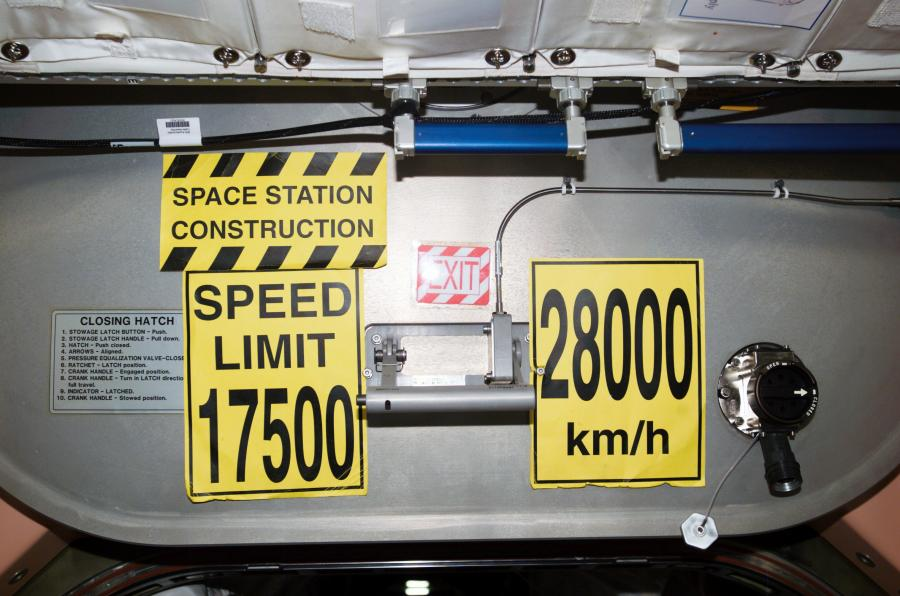
\includegraphics[width=0.9\textwidth]{speed.jpg}
	\end{center}
\end{frame}

\begin{frame}{Stack and Heap Allocation}
	Interior types
	\begin{itemize}
		\item In functional languages, nested datatypes use GC'ed intermediate pointers.
		\item In Rust, they are nested directly.
	\end{itemize}
	\pause
	\linegap

	Rust has \texttt{malloc()} but not \texttt{free()}.
	\begin{itemize}
		\item \texttt{Type*} is spelled \texttt{\textasciitilde{}Type}
		\item \texttt{malloc(expr)} is spelled \texttt{\textasciitilde{}expr}
		\item Values are freed automatically when they go out of scope.
	\end{itemize}
	\pause
	\linegap
	\texttt{\textasciitilde{}Type} pointers are called {\em owned} pointers - more on them later.
\end{frame}

\begin{frame}{Garbage Collection}
	Garbage-collected pointers are spelled \texttt{@Type} and \texttt{@expr}.
	\begin{itemize}
		\item If you don't see ``\texttt{@}'', then you have no GC.
	\end{itemize}
	\pause
	\linegap

	Why make GC optional?
	\begin{itemize}
		\item \textbf{Predictability}: avoiding GC pauses
		\begin{itemize}
			\item Mobile apps, game engines, graphics
		\end{itemize}
		\item \textbf{Concurrency}: Memory-disjoint tasks
		\begin{itemize}
			\item GC is task-local; can't message-pass GC'ed data
			\item (State-of-the-art concurrent GC imposes read/write overhead$^{\small \text{[Tene '11]}}$)
		\end{itemize}
		\item \textbf{Compatibility}: ``Runtime-less'' Rust
		\begin{itemize}
			\item C++ app modules, linux kernel modules, even entire kernels.
		\end{itemize}
	\end{itemize}
\end{frame}

%%%%%%%%%%%%%%%%%%%%%%%%%%%%%%%%%%%%%%%%%%%%%%%%%%%%%%%%%%%%%%%%%%%%%%%%%%%%%%%%
\section{Memory Safety}
%%%%%%%%%%%%%%%%%%%%%%%%%%%%%%%%%%%%%%%%%%%%%%%%%%%%%%%%%%%%%%%%%%%%%%%%%%%%%%%%

\begin{frame}{Safety}
	\begin{center}
	
\includegraphics[width=0.9\textwidth]{safety.jpg}
	\end{center}
\end{frame}

\newcommand\hashtableexample{\begin{tabular}{l}
		\texttt{HashTable<K,V> *table = ...;} \\
		\texttt{foreach value in table \{ \hilight{darkcyan}{// create alias into table}} \\
		\texttt{~~~~table.insert(...); \hilight{darkcyan}{// might reallocate bucket array}} \\
		\texttt{~~~~access(*value);} \\
\texttt{\}}
	\end{tabular} }

\begin{frame}{Motivation: Data Structure Mutation}
	\hashtableexample
	\pause
	\linegap

	\begin{itemize}
		\item \textbf{Go, SML, Haskell}: OK thanks to garbage collection
			\begin{itemize}
				\item (which we wish to avoid)
			\end{itemize}
		\pause
		\item \textbf{C, C++}: Use-after-free
			\begin{itemize}
				\item Mozilla bug \#810718 (CVE-2012-4181) - arbitrary code exec in firefox
			\end{itemize}
		\pause
		\item \textbf{Java}: \texttt{ConcurrentModificationException}
			\begin{itemize}
				\item Run-time failure - can we do better?
			\end{itemize}
	\end{itemize}
\end{frame}

\subsection{Pointers and Ownership}

\begin{frame}{Owned pointers}
	``Owned'' pointers (\texttt{\textasciitilde{}expr}, \texttt{\textasciitilde{}Type}) are noncopyable.
	\begin{itemize}
		\item Hence, they never alias each other.
		\item They must be {\em moved} as arguments.
	\end{itemize}
	\pause
	\linegap
	\begin{tabular}{l}
		\texttt{\hilight{brown}{let}~x~=~\textasciitilde{}\hilight{brickred}{31337};~\hilight{darkcyan}{//~allocate~owned~pointer~to~an~int}} \\
		\texttt{move\_away(x);} \\
		\texttt{\hilight{blue}{printf!}(\hilight{brickred}{"\%d"},~*x);~\hilight{darkcyan}{//~ERROR:~x~was~moved}} \\
		\texttt{} \\
		\texttt{\hilight{brown}{fn}~move\_away(x:~\textasciitilde{}\hilight{olivegreen}{int})~\{} \\
		\texttt{~~~~...~\hilight{darkcyan}{//~x~will~be~freed~by~callee}} \\
		\texttt{\}} \\

	\end{tabular}
\end{frame}

\begin{frame}{Borrowed pointers}
	``Borrowed'' pointers (\texttt{\&expr}, \texttt{\&Type}) can be copied
	\begin{itemize}
		\item Creating one does not allocate
		\item At runtime, same representation as C++ references
		\item Always valid, usage restricted by static {\em lifetime analysis} $^{\small \text{Jim '02}}$
	\end{itemize}
	\pause
	\linegap

	\begin{tabular}{l}
		\texttt{\hilight{brown}{let}~x~=~\textasciitilde{}\hilight{brickred}{31338};} \\
		\texttt{\hilight{brown}{let}~y~=~\&*x;~\hilight{darkcyan}{//~borrow~x}} \\
		\texttt{move\_away(x);~\hilight{darkcyan}{//~ERROR:~cannot~move~x~while~it~is~borrowed}} \\
		\texttt{\hilight{blue}{printf!}(\hilight{brickred}{"\%d"},~*y);} \\

	\end{tabular}
	\pause
	\linegap

	\begin{tabular}{l}
		\texttt{\hilight{brown}{fn}~foo()~->~\&\hilight{olivegreen}{int}~\{} \\
		\texttt{~~~~\hilight{brown}{let}~x~=~\hilight{brickred}{31339};} \\
		\texttt{~~~~\hilight{brown}{let}~y~=~\&x;~\hilight{darkcyan}{//~borrow~x}} \\
		\texttt{~~~~\hilight{brown}{return}~y;~\hilight{darkcyan}{//~ERROR:~y~cannot~outlive~lifetime~of~x}} \\
	\texttt{\}} \\
	\end{tabular}
\end{frame}

\subsection{Mutability}

\begin{frame}{Mutability}
	Mutability must be declared explicitly.
	\begin{itemize}
		\item \texttt{\hilight{brown}{let}~\hilight{brown}{mut}~x~=~\textasciitilde{}[\hilight{brickred}{0},\hilight{brickred}{0},\hilight{brickred}{0}];}
	\end{itemize}
	Mutability is {\em inherited}.
	\begin{itemize}
		\item \texttt{x = ~\textasciitilde{}[\hilight{brickred}{1},\hilight{brickred}{2},\hilight{brickred}{3}];}
		\item \texttt{x[\hilight{brickred}{2}]~=~\hilight{brickred}{4};}
	\end{itemize}
	\pause
	\linegap

	Borrowed pointers can also be mutable (\texttt{\&\hilight{brown}{mut}~expr}, \texttt{\&\hilight{brown}{mut}~Type})
	\begin{itemize}
		\item Mutable borrowed pointers are the {\em only mutable path} to the data.
		\item Cannot coexist with any other borrowed pointer to the same data.
	\end{itemize}
	\pause
	\linegap
	\begin{tabular}{l}
	\texttt{\hilight{brown}{let}~y~=~\&x[\hilight{brickred}{2}];} \\
		\texttt{(\&\hilight{brown}{mut}~x).push(\hilight{brickred}{8});~~\hilight{darkcyan}{//~might~reallocate~the~vector~(ERROR)}} \\
	\texttt{\hilight{blue}{printf!}(\hilight{brickred}{"\%d"},~*y);~\hilight{darkcyan}{//~potential~use-after-free}} \\
	\end{tabular}
\end{frame}

\begin{frame}{Putting it all together}
	Recall:
	\linegap

	\hashtableexample
\end{frame}
\begin{frame}{Putting it all together}
	\begin{tabular}{l}
		\texttt{\hilight{brown}{fn}~each<K,V>(table:~\&\hilight{olivegreen}{HashTable}<K,V>,~f:~\hilight{brown}{fn}(\&K,~\&V))} \\
		\texttt{\hilight{brown}{fn}~insert<K,V>(table:~\&\hilight{brown}{mut}~\hilight{olivegreen}{HashTable}<K,V>,~key:~K,~value:~V)} \\
		\pause
		\texttt{} \\
		\texttt{\hilight{brown}{let}~table~=~...;} \\
		\texttt{} \\
		\texttt{} \\
		\texttt{\hilight{brown}{do}~(\&table).each~|key,value|~\{} \\
		\texttt{} \\
		\texttt{} \\
		\texttt{~~~~(\&\hilight{brown}{mut}~table).insert(...);~} \\
		\texttt{} \\
		\texttt{~~~~\hilight{blue}{printf!}(\hilight{brickred}{"\%?"},~*value);} \\
		\texttt{\}} \\

	\end{tabular}
\end{frame}
\begin{frame}{Putting it all together}
	\begin{tabular}{l}
		\texttt{\hilight{brown}{fn}~each<K,V>(table:~\&\hilight{olivegreen}{HashTable}<K,V>,~f:~\hilight{brown}{fn}(\&K,~\&V))} \\
		\texttt{\hilight{brown}{fn}~insert<K,V>(table:~\&\hilight{brown}{mut}~\hilight{olivegreen}{HashTable}<K,V>,~key:~K,~value:~V)} \\
		\texttt{} \\
		\texttt{\hilight{brown}{let}~table~=~...;} \\
		\texttt{} \\
		\texttt{\hilight{darkcyan}{//~NOTE:~prior~borrow~occurred~here}} \\
		\texttt{\hilight{brown}{do}~(\&table).each~|key,value|~\{} \\
		\texttt{~~~~\hilight{darkcyan}{//~ERROR:~cannot~borrow~`table'~as~mutable~due~to}} \\
		\texttt{~~~~\hilight{darkcyan}{//~conflicting~prior~borrow}} \\
		\texttt{~~~~(\&\hilight{brown}{mut}~table).insert(...);~} \\
		\texttt{} \\
		\texttt{~~~~\hilight{blue}{printf!}(\hilight{brickred}{"\%?"},~*value);} \\
		\texttt{\}} \\

	\end{tabular}
\end{frame}

%%%%%%%%%%%%%%%%%%%%%%%%%%%%%%%%%%%%%%%%%%%%%%%%%%%%%%%%%%%%%%%%%%%%%%%%%%%%%%%%
\section{Concurrency}
%%%%%%%%%%%%%%%%%%%%%%%%%%%%%%%%%%%%%%%%%%%%%%%%%%%%%%%%%%%%%%%%%%%%%%%%%%%%%%%%

\begin{frame}{Concurrency}
	\begin{center}
	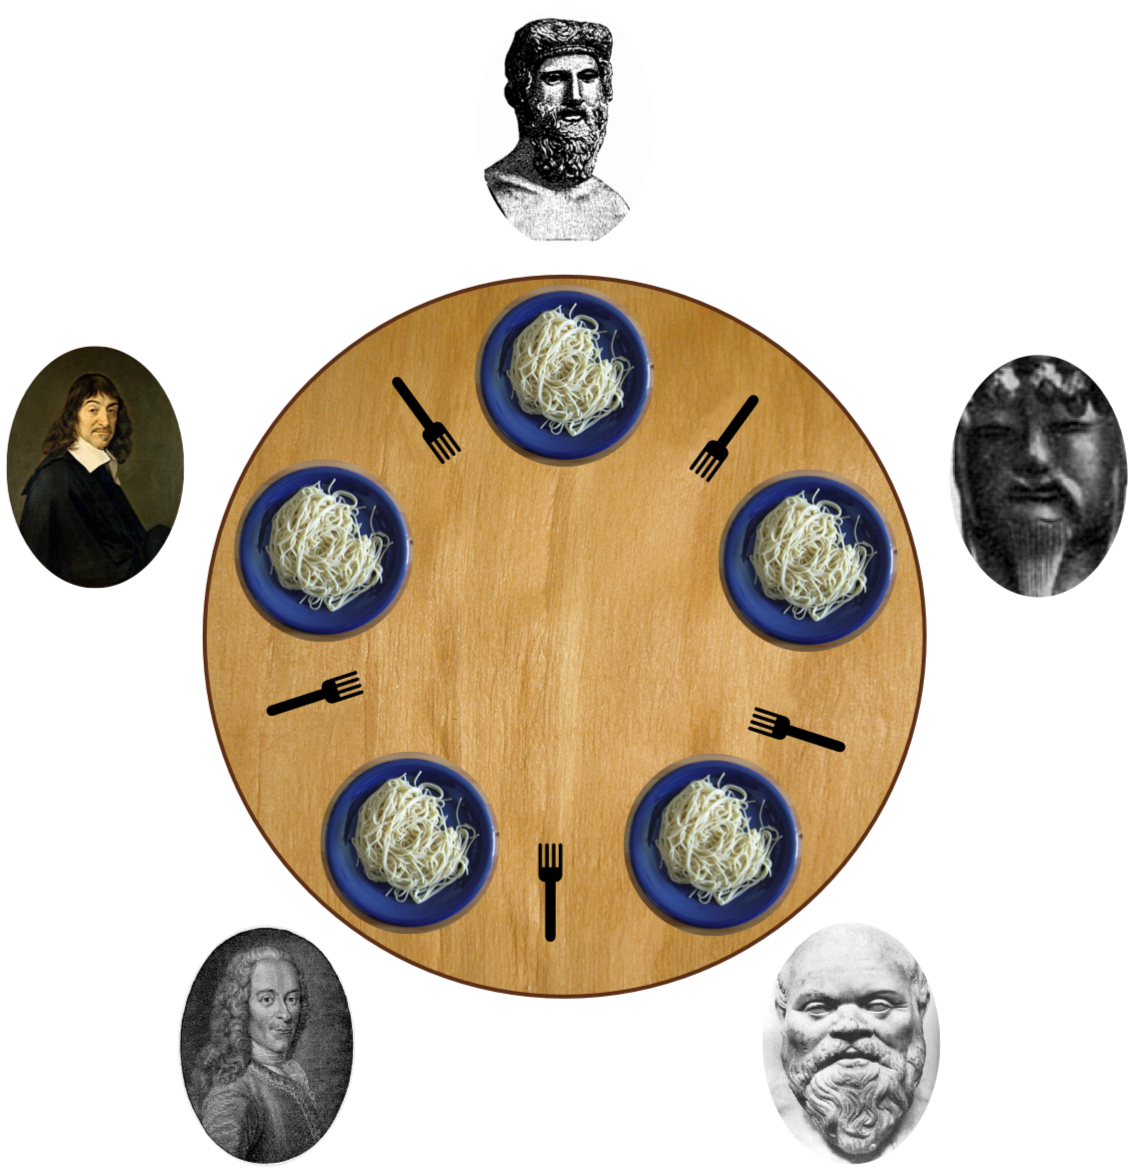
\includegraphics[width=0.6\textwidth]{concurrency.jpg}
	\end{center}
\end{frame}

%make sure before this to talk about noncopyability and moving
\subsection{Tasks}

\begin{frame}{Data Races}
        Data race: Concurrent access where at least one is a write.$^{\small \text{[Savage '97]}}$
        \linegap

        Go's mutable global state can be used to break type safety and crash.
        \begin{itemize}
                \item \texttt{http://research.swtch.com/gorace} (Feb '10)
                \item \texttt{http://blog.golang.org/race-detector} (June '13)
        \end{itemize}
        \pause
        \linegap

        Rust forbids global mutable state.
        \begin{itemize}
                \item Tasks must communicate via message-passing.
		\item Type system ensures this is safe (which I will now justify).
        \end{itemize}
\end{frame}

\begin{frame}{Kinds of Types}
        Rust compiler automatically determines what {\em kinds} each type has.
        \pause
        \linegap

        The \texttt{\hilight{violet}{Send}} kind
        \begin{itemize}
                \item A \texttt{\hilight{violet}{Send}}able type cannot alias any memory owned elsewhere.
                \item No \texttt{\&}-pointers
                \item No \texttt{@}-pointers
                \item Moving a \texttt{\hilight{violet}{Send}}able type into another task gives up access rights to its memory.
        \end{itemize}
        \pause
        \linegap
        Examples: \\
        \begin{tabular}{l}
		\texttt{\hilight{darkcyan}{//~sendable}} \\
		\texttt{\hilight{brown}{struct}~\hilight{olivegreen}{Foo}~\{} \\
			\texttt{~~~~x:~\hilight{olivegreen}{int},} \\
			\texttt{~~~~y:~\textasciitilde{}[\hilight{olivegreen}{bool}],} \\
		\texttt{\}}
        \end{tabular}
        \quad
        \begin{tabular}{l}
		\texttt{\hilight{darkcyan}{//~depends~on~T}} \\
		\texttt{\hilight{brown}{struct}~\hilight{olivegreen}{Bar}<T>~\{} \\
			\texttt{~~~~t:~T,} \\
			\texttt{~~~~f:~\hilight{olivegreen}{Foo},} \\
		\texttt{\}}
        \end{tabular}
        \quad
        \begin{tabular}{l}
		\texttt{\hilight{darkcyan}{//~NOT~sendable}} \\
		\texttt{\hilight{brown}{struct}~\hilight{olivegreen}{Baz}~\{} \\
			\texttt{~~~~p:~\&\hilight{olivegreen}{int},} \\
		\texttt{\}} \\
		\texttt{}
        \end{tabular}
\end{frame}

\begin{frame}{Spawning and Sending}
        Type signature of \texttt{spawn}:
        \begin{itemize}
                \item \texttt{\hilight{brown}{fn}~spawn(task\_body:~\textasciitilde{}\hilight{brown}{fn}())}
                \item \texttt{\textasciitilde{}\hilight{brown}{fn}()} means a {\em heap-allocated} closure
                \begin{itemize}
                        \item Environment can only capture \texttt{\hilight{violet}{Send}}able types.
                \end{itemize}
        \end{itemize}
        \pause
        \linegap

        Type signature of message-passing:
        \begin{itemize}
		\item \texttt{\hilight{brown}{fn}~send<T:~\hilight{violet}{Send}>(chan:~\hilight{olivegreen}{Chan}<T>,~data:~T)}
		\item \texttt{\hilight{brown}{fn}~recv<T:~\hilight{violet}{Send}>(port:~\hilight{olivegreen}{Port}<T>)~->~T}
        \end{itemize}
        \pause
        \linegap
        It follows that tasks can never alias the same memory, hence no data races.
\end{frame}

\begin{frame}{Freezing and Sharing}
        Goal: restore ability to share without compromising data-race freedom.
        \pause
        \linegap

        The \texttt{\hilight{violet}{Freeze}} kind
	\begin{itemize}
		\item A \texttt{\hilight{violet}{Freeze}}able type contains no {\em internal mutability}
		\item No \texttt{\&\hilight{brown}{mut}~T} pointers
		\item No library types with internal mutability
		\item If \texttt{ptr:~\&T} and \texttt{T: \hilight{violet}{Freeze}}, then \texttt{ptr} is {\em deeply immutable}.
	\end{itemize}
\end{frame}

\begin{frame}{Freezing and Sharing}
	\textbf{RWArc}: ``Reader/writer atomically-reference-counted object''
	\begin{itemize}
		\item Can alias freezable data between tasks using an R/W lock.
		\item Type system enforces the lock must be held in the correct mode.
	\end{itemize}
	\pause
	\linegap
	\begin{tabular}{l}
		\texttt{\hilight{darkcyan}{//~Move~freezable~data~into~an~RWArc~wrapper.}} \\
		\texttt{\hilight{brown}{fn}~new<T:~\hilight{violet}{Send}+\hilight{violet}{Freeze}>(data:~T)~->~\hilight{olivegreen}{RWArc}<T>} \\
		\pause
		\texttt{} \\
		\texttt{\hilight{darkcyan}{//~Make~a~new~handle~to~the~data,~incrementing~the~refcount.}} \\
		\texttt{\hilight{brown}{fn}~clone<T:~\hilight{violet}{Send}+\hilight{violet}{Freeze}>(handle:~\&\hilight{olivegreen}{RWArc}<T>)~->~\hilight{olivegreen}{RWArc}<T>} \\
		\pause
		\texttt{} \\
		\texttt{\hilight{darkcyan}{//~Get~an~immutable~reference~with~the~lock~in~`read'~mode.}} \\
		\texttt{\hilight{brown}{fn}~read~<T:~\hilight{violet}{Send}+\hilight{violet}{Freeze}>(handle:~\&\hilight{olivegreen}{RWArc}<T>,~f:~\hilight{brown}{fn}(\&T))} \\
		\pause
		\texttt{} \\
		\texttt{\hilight{darkcyan}{//~Get~a~mutable~reference~with~the~lock~in~`write'~mode.}} \\
		\texttt{\hilight{brown}{fn}~write<T:~\hilight{violet}{Send}+\hilight{violet}{Freeze}>(handle:~\&\hilight{olivegreen}{RWArc}<T>,~f:~\hilight{brown}{fn}(\&\hilight{brown}{mut}~T))} \\
	\end{tabular}
\end{frame}

%%%%%%%%%%%%%%%%%%%%%%%%%%%%%%%%%%%%%%%%%%%%%%%%%%%%%%%%%%%%%%%%%%%%%%%%%%%%%%%%
\section{Conclusion}
%%%%%%%%%%%%%%%%%%%%%%%%%%%%%%%%%%%%%%%%%%%%%%%%%%%%%%%%%%%%%%%%%%%%%%%%%%%%%%%%

\begin{frame}{Conclusion}
	Rust achieves:
	\begin{itemize}
		\item Systems-level performance demands
		\item Memory safety in the face of mutable aliases
		\item Data-race-free concurrency
	\end{itemize}
	\linegap

	through the use of:
	\begin{itemize}
		\item Ownership (linear/noncopyable) types
		\item Static lifetime analysis (borrow-checking)
		\item Kind analysis and safe concurrency library interfaces
	\end{itemize}
\end{frame}

\begin{frame}{Questions?}
	% rust logo
	\begin{center}
		
\includegraphics[width=0.6\textwidth]{rust.png}
	\end{center}
\end{frame}

% \begin{frame}{Bonus slides}
% 	\begin{center}
% 	\large \textit{(I'm glad you asked that\dots)}
% 	\end{center}
% \end{frame}
%
% \begin{frame}{Sharing Mutable State}
% 	\textbf{``RW-Arc'':} reader-/writer-locked atomically-refcounted shared state.
% 	\code {
% 		\texttt{\hilight{brown}{impl}~<T:~\hilight{violet}{Freeze}+\hilight{violet}{Send}>~\&\hilight{olivegreen}{RWArc}<T>~\{} \\
% \texttt{~~~~\hilight{brown}{fn}~\hilight{olivegreen}{read}~~(blk:~\hilight{brown}{fn}(\&T))~...} \\
% \texttt{~~~~\hilight{brown}{fn}~\hilight{olivegreen}{write}~(blk:~\hilight{brown}{fn}(\&\hilight{brown}{mut}~T))~...} \\
% %\texttt{~~~~\hilight{brown}{fn}~\hilight{olivegreen}{write\_cond}(blk:~\hilight{brown}{fn}(\&\hilight{brown}{mut}~T,~\&condvar));} \\
% \texttt{\}} \\
% 	}
% %		impl <T: const send> &rw_arc<T> {
% %		    fn read      (blk: fn(&T));
% %		    fn write     (blk: fn(&mut T));
% %		    fn write_cond(blk: fn(&mut T, &condvar));
% %		}
%
% 	\begin{center}
% 	\begin{tabular}{cc}
% 		\begin{tabular}{l}
% %\texttt{\hilight{brown}{do}~arc.write\_cond~|state,c|~\{} \\
% \texttt{\hilight{brown}{do}~arc.write~|state:~\&\hilight{brown}{mut}~T|~\{} \\
% \texttt{~~~~\hilight{darkcyan}{//~exclusive~access;}} \\
% %\texttt{~~~~c.wait();} \\
% \texttt{~~~~\hilight{darkcyan}{//~can~modify~the~data}} \\
% \texttt{~~~~*state~=~\hilight{brickred}{17};} \\
% %\texttt{~~~~c.signal();} \\
% \texttt{\}} \\
% 		\end{tabular}
% 	&
% %		do arc.write_cond |state, cond| {
% %		    // exclusive access
% %		    cond.wait();    // can block...
% %		    *state = 17;    // modify the data...
% %		    cond.signal();  // and wake others
% %		}
% 		\begin{tabular}{l}
% \texttt{\hilight{brown}{do}~arc.read~|state:~\&T|~\{} \\
% \texttt{~~~~\hilight{darkcyan}{//~concurrent~access}} \\
% \texttt{~~~~\hilight{darkcyan}{//~immutable~state}} \\
% \texttt{~~~~\hilight{red}{assert}~*state~==~\hilight{brickred}{17};} \\
% \texttt{~~~~\hilight{darkcyan}{//~won't~compile}} \\
% \texttt{~~~~\hilight{darkcyan}{//~*state += 1;}} \\
% \texttt{\}} \\
% 		\end{tabular}
% 	\end{tabular}
% 	\end{center}
% %		do arc.read |state| {
% %		    // shared access - immutable state
% %		    assert *state == 17;  // OK
% %		    *state += 1;  // Won't compile
% %		}
% \end{frame}

\end{document}

%%%%%%%%%%%%%%%%%%%%%%%%%%%%%%%%%%%%%%%%%%%%%%%%%%%%%%%%%%%%%%%%%%%%%%%%%%%%%%%%
% vim: foldmethod=indent
